\documentclass{article}

\usepackage[utf8]{inputenc} % allow utf-8 input
\usepackage[T1]{fontenc}    % use 8-bit T1 fonts
\usepackage{hyperref}       % hyperlinks
\usepackage{url}            % simple URL typesetting
\usepackage{booktabs}       % professional-quality tables
\usepackage{amsfonts}       % blackboard math symbols
\usepackage{nicefrac}       % compact symbols for 1/2, etc.
\usepackage{microtype}      % microtypography
\usepackage{xcolor}         % colors
\usepackage{amssymb}
\usepackage{float}
\usepackage{graphicx} 
\usepackage{stmaryrd}       % double square brackets |[ ]|
\usepackage{amsmath}        % \underset for argmax
\usepackage{changepage}     % adjust figure width


\title{Financial Document Analysis: Checkpoint 1}

\begin{document}

\maketitle


\section{SEC EDGAR Data}

\subsection{What is SEC-EDGAR?}


\subsection{iXBRL Annotation Systems}
In EDGAR, the iXBRL provided by various submitting entities uses multiple annotation systems. The most prominent of these systems is 'us-gaap'. Many companies have embraced iXBRL as early adopters in the SEC-EDGAR database, although formal requirements for adoption are being phased in for the future. We see that each studied company has added internal iXBRL tags that are parseable in their submitted documents.

\begin{center}
\includegraphics[width=\linewidth]{share_anno_tags_pie.png}
\end{center}


\subsection{Annotation Adoption by Company}
In this section, we consider iXBRL labels by how often companies adopt them in their documents. First we remove all company-specific iXBRL schemes, and we consider what share of companies use each unique iXBRL tag in the dataset.

\begin{center}
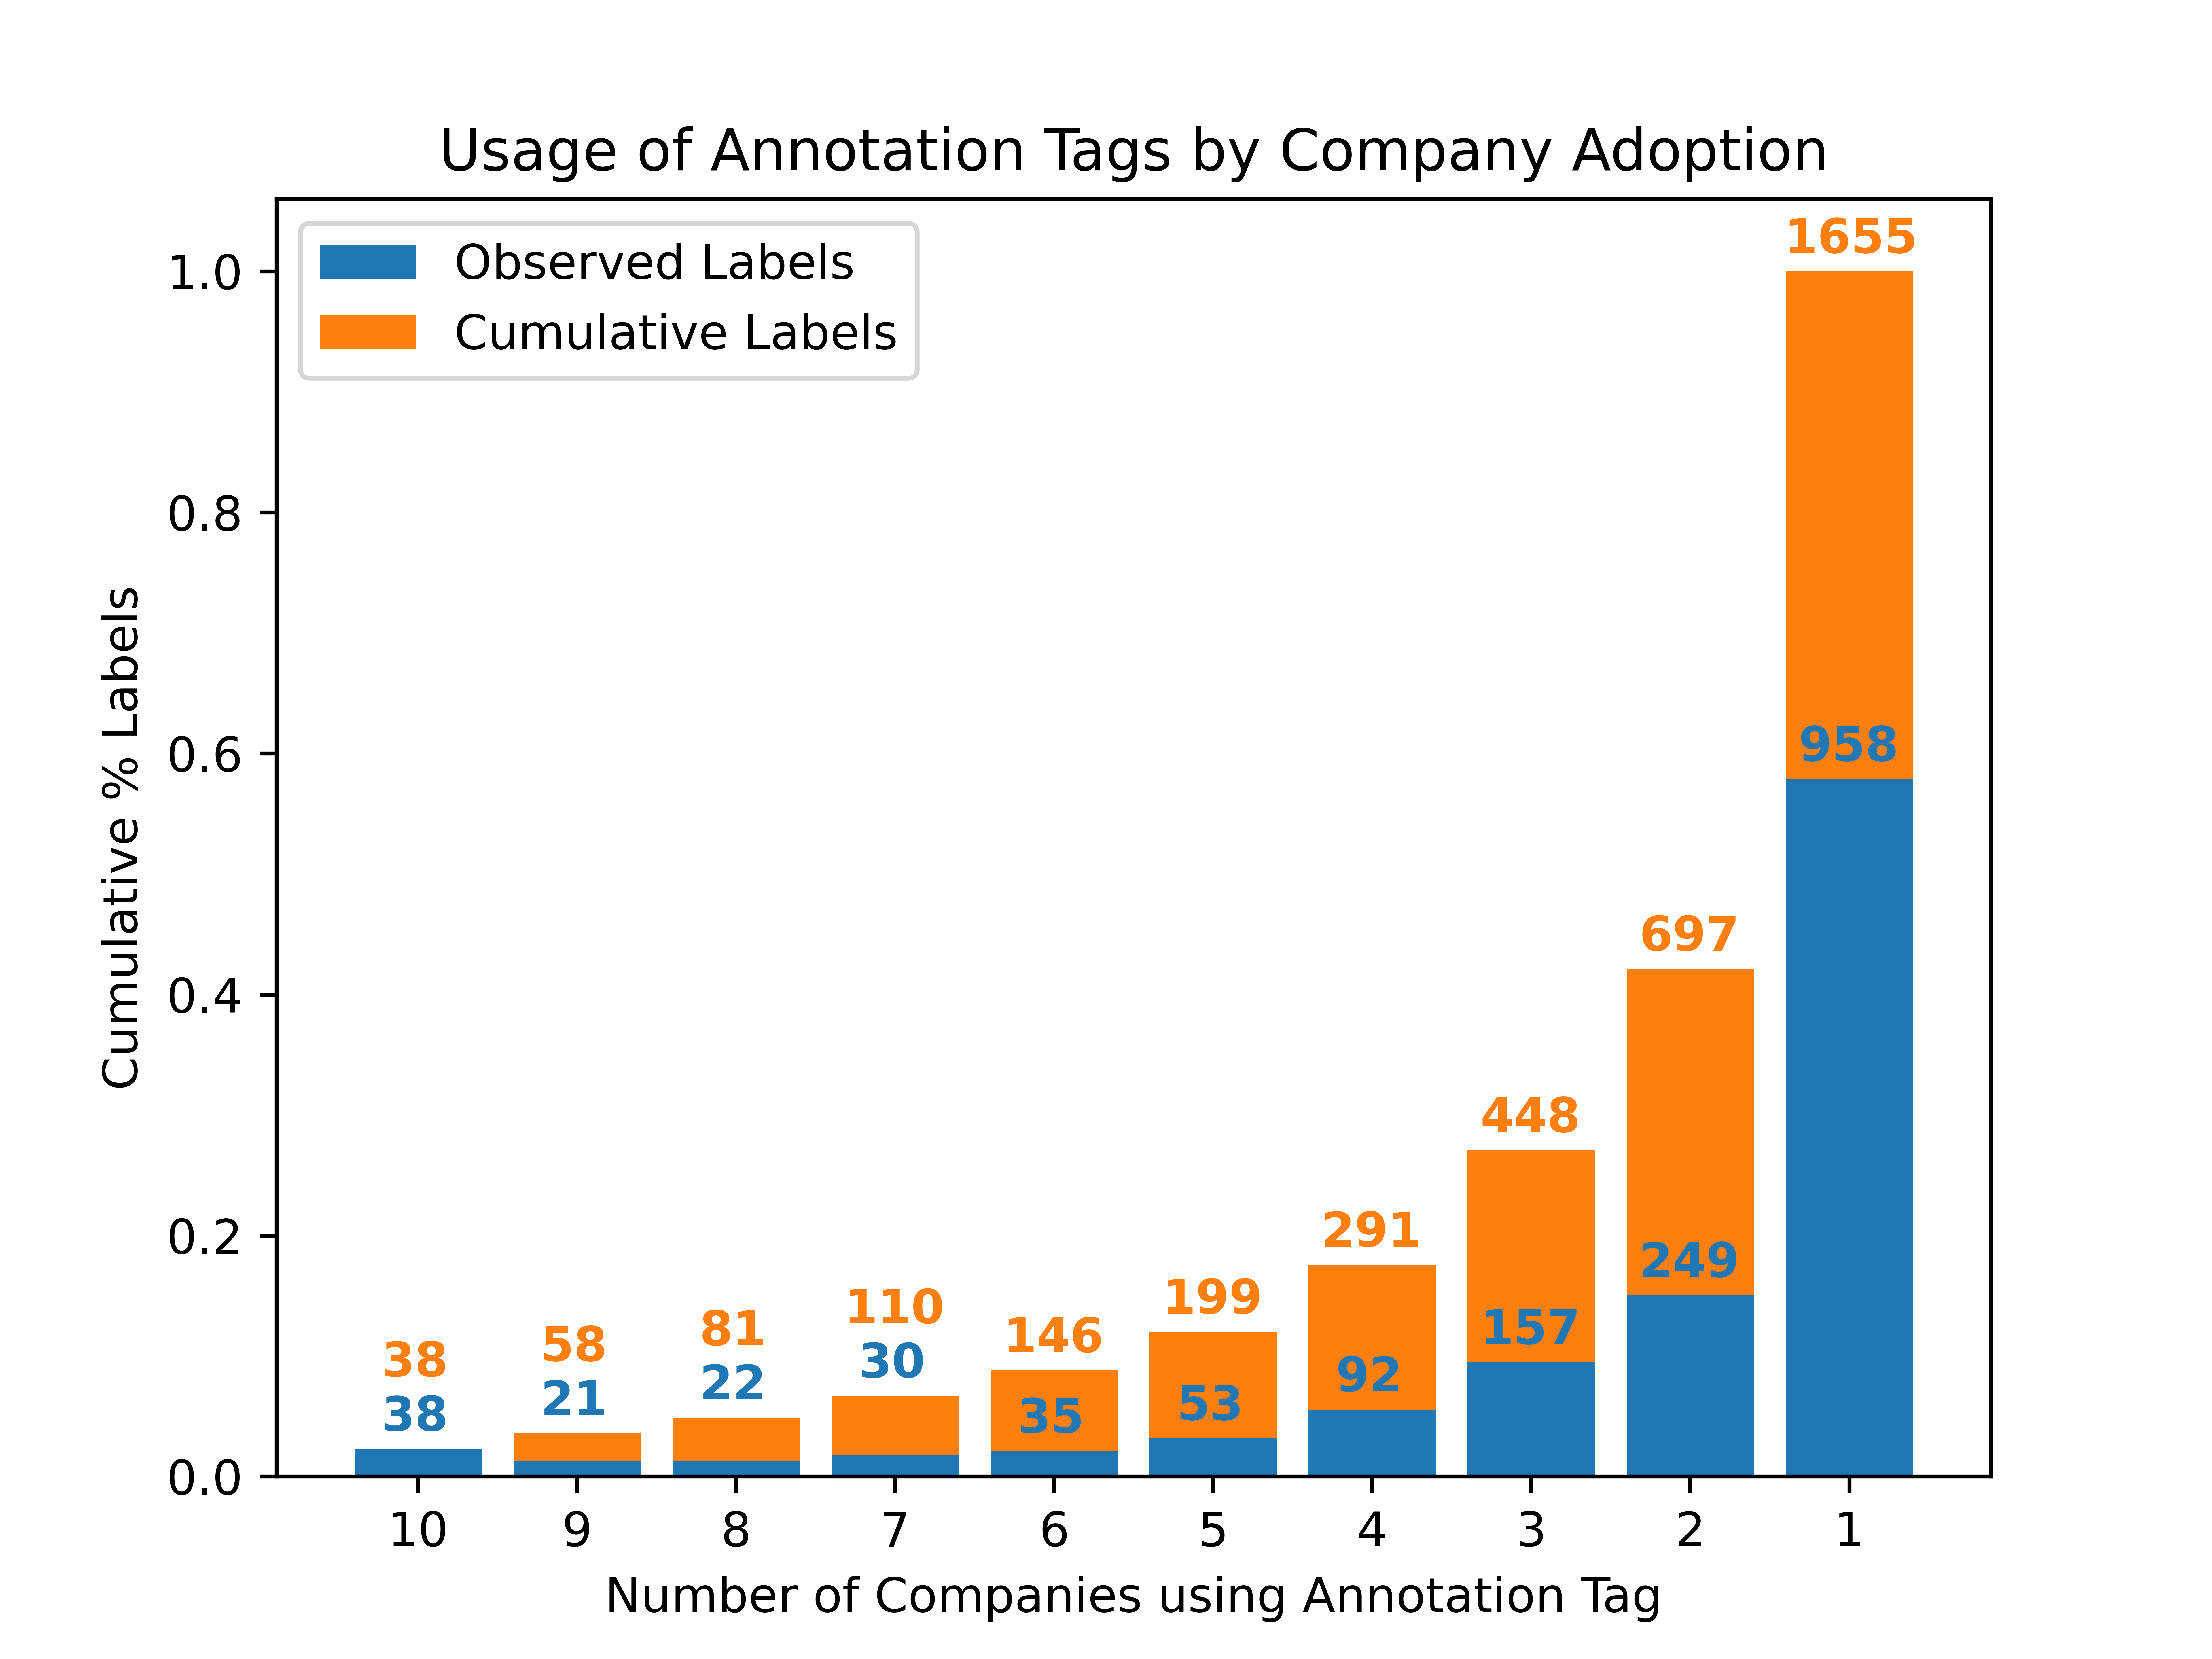
\includegraphics[width=\linewidth]{anno_coverage_vs_company_adoption.png}
\end{center}
Even after filtering out company-specific iXBRL system annotations, we are left with many unique 'us-gaap' annotations that are not widely adopted by most companies. Most 'us-gaap' standard annotations are used by one reporting company, and only a small minority (38) are used by all reported companies.

\end{document}
